% Hlavicka pro protokoly z fyzikalniho praktika.
% Verze pro: LaTeX
% Verze hlavicky: 22. 2. 2007
% Autor: Ustav fyziky kondenzovanych latek
% Ke stazeni: www.physics.muni.cz/ufkl/Vyuka/
% Licence: volne k pouziti, nejlepe k vcasnemu odevzdani protokolu z Vaseho mereni.

\documentclass[a4paper,11pt]{article}

% Kodovani (cestiny) v dokumentu: utf-8
%\usepackage[cp1250]{inputenc}	% Omezena stredoevropska kodova stranka, pouze MSW.
\usepackage[utf8]{inputenc}	% Doporucujeme pouzivat UTF-8 (unicode).

%%% Nemente:
\usepackage[margin=2cm]{geometry}
\newtoks\jmenopraktika \newtoks\jmeno \newtoks\datum
\newtoks\obor \newtoks\skupina \newtoks\rocnik \newtoks\semestr
\newtoks\cisloulohy \newtoks\jmenoulohy
\newtoks\tlak \newtoks\teplota \newtoks\vlhkost
\usepackage{amsmath}
\usepackage{mathtools}
\usepackage{graphicx}
\usepackage{multirow}
\graphicspath{ {./images/} }
%%% Nemente - konec.


%%%%%%%%%%% Doplnte pozadovane polozky:

\jmenopraktika={Fyzikální praktikum 2}  % nahradte jmenem vaseho predmetu
\jmeno={Artem Gorodilov}            % nahradte jmenem mericiho
\datum={26. ~října  2023}        % nahradte datem mereni ulohy
\obor={Astrofyzika}                     % nahradte zkratkou vami studovaneho oboru
\skupina={Čt 8:00}            % nahradte dobou vyuky vasi seminarni skupiny
\rocnik={II}                  % nahradte rocnikem, ve kterem studujete
\semestr={I}                 % nahradte semestrem, ve kterem studujete

\cisloulohy={6}               % nahradte cislem merene ulohy
\jmenoulohy={Elektromagnetické kmity v RLC obvodu} % nahradte jmenem merene ulohy

\tlak={987}                   % nahradte tlakem pri mereni (v hPa)
\teplota={21.1}               % nahradte teplotou pri mereni (ve stupnich Celsia)
\vlhkost={41}               % nahradte vlhkosti vzduchu pri mereni (v %)

%%%%%%%%%%% Konec pozadovanych polozek.


%%%%%%%%%%% Uzitecne balicky:
\usepackage[czech]{babel}
\usepackage{graphicx}
\usepackage{amsmath}
\usepackage{xspace}
\usepackage{url}
\usepackage{indentfirst}
\usepackage{listings}
\usepackage{subcaption}
\usepackage{caption}
\usepackage{tabularx}
\usepackage[labelformat=parens,labelsep=quad,skip=3pt]{caption}

%%%%%% Zamezeni parchantu:
\widowpenalty 10000 \clubpenalty 10000 \displaywidowpenalty 10000
%%%%%% Parametry pro moznost vsazeni vetsiho poctu obrazku na stranku
\setcounter{topnumber}{3}	  % max. pocet floatu nahore (specifikace t)
\setcounter{bottomnumber}{3}	  % max. pocet floatu dole (specifikace b)
\setcounter{totalnumber}{6}	  % max. pocet floatu na strance celkem
\renewcommand\topfraction{0.9}	  % max podil stranky pro floaty nahore
\renewcommand\bottomfraction{0.9} % max podil stranky pro floaty dole
\renewcommand\textfraction{0.1}	  % min podil stranky, ktery musi obsahovat text
\intextsep=8mm \textfloatsep=8mm  %\intextsep pro ulozeni [h] floatu a \textfloatsep pro [b] or [t]

% Tecky za cisly sekci:
\renewcommand{\thesection}{\arabic{section}.}
\renewcommand{\thesubsection}{\thesection\arabic{subsection}.}
% Jednopismenna mezera mezi cislem a nazvem kapitoly:
\makeatletter \def\@seccntformat#1{\csname the#1\endcsname\hspace{1ex}} \makeatother

\begin{document}

\thispagestyle{empty}

{
\begin{center}
\sf 
{\Large Ústav fyzikální elektroniky PřF MU} \\
\bigskip
{\huge \bfseries FYZIKÁLNÍ PRAKTIKUM} \\
\bigskip
{\Large \the\jmenopraktika}
\end{center}

\bigskip

\sf
\noindent
\setlength{\arrayrulewidth}{1pt}
\begin{tabular*}{\textwidth}{@{\extracolsep{\fill}} l l}
\large {\bfseries Zpracoval:}  \the\jmeno & \large  {\bfseries Naměřeno:} \the\datum\\[2mm]
\large  {\bfseries Obor:} \the\obor  \hspace{40mm}  {\bfseries Skupina:} \the\skupina %
%{\bfseries Ročník:} \the\rocnik \hspace{5mm} {\bfseries Semestr:} \the\semestr  
&\large {\bfseries Testováno:}\\
\\
\hline
\end{tabular*}
}

\bigskip

{
\sf
\noindent \begin{tabular}{p{3cm} p{0.6\textwidth}}
\Large  Úloha č. {\bfseries \the\cisloulohy:} \par
\smallskip
$T=\the\teplota$~$^\circ$C \par
$p=\the\tlak$~hPa \par
$\varphi=\the\vlhkost$~\%
&\Large \bfseries \the\jmenoulohy  \\[2mm]
\end{tabular}
}

\vskip1cm
\begin{minipage}[t]{1\textwidth}
    \section{Zadání}
        Určit impedanci rezistoru, cívky a kondenzátoru. 
        \par Změřit frekvenční charakteristiku RLC obvodu a na jejím základě zjistit odpor, kapacitu a indukčnost.
        \par Změřit přechodové jevy při podkritickém, kritickém a nadkritickém tlumení.
\end{minipage}
    \par
\vspace{10px}
\begin{minipage}[t]{0.5\textwidth} 
    \section{Teorie}
        $RLC$ obvod se skládá z rezistoru s hodnotou $R$, cívky s indukčností $L$ a kondenzátoru s kapacitou $C$, které jsou buď zapojeny sériově nebo paralelně. Při buzení těchto obvodů střídavým napětím při určité frekvenci dochází k rezonanci, která je charakterizována maximálním proudem. Podobné rezonanční chování lze pozorovat v různých oblastech fyziky, například při působení periodické síly na závaží připevněné k pružině. Obvody s rezistorem, cívkou a kondenzátorem mají široké využití jako rezonátory, filtry s horní a dolní propustí nebo integrační členy.
        \subsection{Impedance}
            Prvně jsme pomocí multimetru provedli přímá měření odporu rezistoru, kapacity kondenzátoru a indukčnosti cívky. Začali jsme sestavením obvodu podle schématu na obrázku (\ref{fig:rlc}). Postupně jsme prováděli měření pro rezistor, kondenzátor a cívku při frekvencích 1 a 30 kHz. Poté jsme přešli k sestavení obvodu s osciloskopem, viz obrázek (\ref{fig:imp1}). Výsledky z osciloskopu nám poskytly informace o rozdílu napětí $U_1$ a $U_2$, fázi a hodnotě $U_2$.
            \par Nejprve jsme využili napětí $U_2$ a referenčního odporu $R_I$, který jsme si sami zvolili, k výpočtu proudu procházejícího obvodem pomocí Ohmova zákona.
\end{minipage}
\hspace{10pt}
\begin{minipage}[t]{0.5\textwidth} 
             Na základě toho jsme ověřili naměřený odpor, který jsme také vypočítali pomocí Ohmova zákona, avšak tentokrát s rozdílem napětí $U_1 - U_2$. Využitím následujícího vztahu zpočítáme absolutní hodnotu impedance $Z$ a jeho fáze $\varphi_Z$:
            \begin{equation}
                \vert Z\vert = R_I \frac{\vert U_1-U_2\vert}{\vert U_2\vert}, ~resp.~ \varphi_Z = \varphi_{M\rightarrow 2}
            \end{equation}
            kde $\vert U_1-U_2\vert$ = $U_{M0}$ a $\vert U_2\vert$ = $U_{20}$.
            \par V případě odporu pak dostáváme pro jeho impedanci $Z_R$:
            \begin{equation}
                Z_R = R = R_R
            \end{equation}
            kde $R_R$ je odpor dekády.
            \vspace{10pt}
            \par \centering
            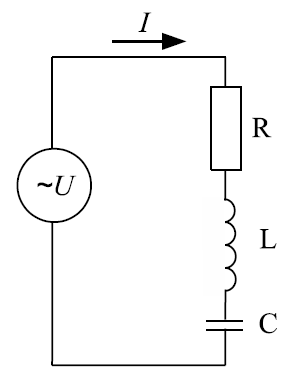
\includegraphics[scale=0.4]{rlc}
            \captionsetup{justification=centering, font=footnotesize}
            \captionof{figure}{Schéma sériového RLC obvodu napájeného zdrojem střídavého napětí U(t).}
            \label{fig:rlc}
            \vspace{10pt}
            \raggedright
            \vspace{10pt}
            \par 
\end{minipage}
\newpage
\begin{minipage}[t]{0.5\textwidth} 
            \centering
            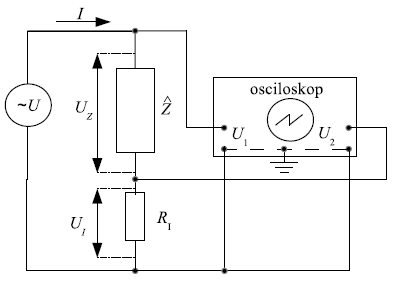
\includegraphics[scale=0.5]{imp1}
            \captionsetup{justification=centering, font=footnotesize}
            \captionof{figure}{Aparatura pro měření impedance $\widehat{Z}$ (nebo vodivosti $\widehat{G} = 1/\widehat{Z}$) zestávající z funkčního generátoru jako zdroje napětí $U$ s určitou frekvencí, osciloskopu, měřené impedance $\widehat{Z}$ a referenčního odporu $R_I$ . V schématu jsou naznačena napětí $U_I$ na referenčním odporu $R_I$ a napětí $U_Z$ na měřené impedanci $Z$. Referenční (stínící) vodiče kanálů $U_1$ a $U_2$ jsou uvnitř osciloskopu spojeny a uzemněny}
            \label{fig:imp1}
            \vspace{10pt}
            \raggedright
            \par Získanou absolutní hodnotu impedance jsme teoreticky využili k ověření kapacity kondenzátoru $C$ pomocí následujícího vztahu:
            \begin{equation}
                C = -\frac{1}{2\pi f \vert Z_C\vert sin\varphi_C}
            \end{equation}
            kde $f$ je frekvenci naměřenou z funkčního generátoru, $Z_C$ je impedance kondenzátoru a $\varphi_C$ je jeho fáze. 
            \par Odpor kondenzátoru $R_C$ se bude rovnat: 
            \begin{equation}
                R_C = Z_C cos\varphi_C
            \end{equation}
            Zjistíme indukci cívky $L$ pomocí vztahu:
            \begin{equation}
                L = \frac{\vert Z_L\vert sin\varphi_L}{2\pi f}
            \end{equation}
            kde $Z_L$ je impedance a $\varphi_L$ je fáze cívky.
            \par Odpor cívky $R_L$ se bude rovnat: 
            \begin{equation}
                R_L = Z_L cos\varphi_L
            \end{equation}
            \par Získané hodnoty jsme použili k výpočtu teoretické hodnoty rezonanční frekvence obvodu $f_0$, pro který jsme využili následující vztah:
            \begin{equation}
                f_0 = \frac{1}{2\pi \sqrt{LC}}
            \end{equation}
        \subsection{Frekvenční charakteristika obvodu RLC}
            Pro měření frekvenčních charakteristik jsme využili předchozí zapojení zobrazené na obrázku (\ref{fig:imp1}). Provedli jsme měření stejných veličin jako v předchozí části, tedy frekvenci, rozdíl napětí $U_1 - U_2$, napětí $U_2$ a fázi v okolí rezonanční frekvence, kterou jsme teoreticky vypočítali v první části.  
\end{minipage}
\hspace{10pt}
\begin{minipage}[t]{0.5\textwidth} 
            \vspace{-100pt}
            \par Měření jsme provedli pro 16 frekvencí, a získané hodnoty jsme použili k výpočtu absolutní hodnoty impedance $\vert Z\vert$ a amplitudy vodivosti $\vert G\vert$. Následně jsme vizualizovali křivky závislosti amplitudy vodivosti na frekvenci a závislosti fáze na frekvenci. 
            \par Rezonanční úhlovou frekvenci $\omega_0$ lze zjistit ze vzorce: 
            \begin{equation}
                \omega_0 = \frac{1}{\sqrt{LC}}
            \end{equation}
            Síla oscilátoru $F$ podle vzorce: 
            \begin{equation}
                F = \frac{1}{L}
            \end{equation}
            Konstanta tlumení $\alpha_0$ se zjistí jako: 
            \begin{equation}
                \alpha_0 = \frac{R}{2L}
            \end{equation}
            A zjistěme koeficient jakosti $Q$:
            \begin{equation}
                Q = \frac{\omega_0}{2 \alpha_0} = \frac{L \omega_0}{R}
            \end{equation}
            \par Následně jsme z absolutní impedance vypočítali amplitudu vodivosti $\vert G\vert$ a jeho fáze $\varphi_G$ podle následujícího vzorce:
            \begin{equation}
                \vert G\vert  = \frac{1}{\vert Z\vert}, ~resp.~ \varphi_G = -\varphi_{M\rightarrow 2}
            \end{equation}
            Z amplitudy vodivosti při rezonanci tak můžeme identifikovat hodnotu odporu $R_{celk}$. V případě reálného $RLC$ obvodu tato rezistence odpovídá celkovým ztrátám v obvodu, které jsou dány součtem ekvivalentních sériových odporů všech komponent na dané frekvenci:
            \begin{equation}
                R_{celk} = R_R + R_L + R_C
            \end{equation}
        \subsection{Přechodný jev RLC obvodu}
            K měření přechodového jevu jsme použili obvod na obrázku (\ref{fig:imp2}). Pro podkritické tlumení je $\alpha_0$ menší než $\omega_0$. Poté jsme provedli přechodová měření pomocí osciloskopu a zpracovali získaná data. Nejprve jsme vykreslili závislost $U_2$ na čase $t$. Poté jsme pomocí maximálních hodnot určili $ln(U_C-U_f)$ (kde $U_C$ je amplituda maxim nebo minim oscilací a $U_f$ je konečné napětí) a vyjádřili jejich lineární závislost z fitu.
            \par Tlumenou kruhovou rezonanční frekvenci  $\omega_d$ lze zjistit ze vzorce:
            \begin{equation}
                \omega_d = \sqrt{\omega_0^2-\alpha^2}
            \end{equation}
\end{minipage}
\newpage
\begin{minipage}[t]{0.5\textwidth} 
            \centering
            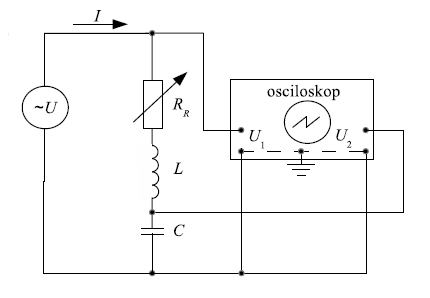
\includegraphics[scale=0.5]{imp2}
            \captionsetup{justification=centering, font=footnotesize}
            \captionof{figure}{Aparatura analogická panelu na obrázku (\ref{fig:imp1}) použitá pro měření přechodového jevu náboje na kondenzátoru $C$.}
            \label{fig:imp2}
            \vspace{10pt}
            \raggedright
            $\omega_0$ pak se bude rovná:
            \begin{equation}
                \omega_0 = \sqrt{\omega_d^2+\alpha^2}
            \end{equation}
            V případě kritického tlumení platí, že $\alpha$ = $\omega_0$. Do obvodu jsme integrovali odporovou dekádu, abychom určili odpor při kritickém tlumení. Následně jsme zaznamenali přechodový jev pro kritické tlumení a naměřená data $U_2$ jsme závislostí na čase interpretovali. Současně jsme teoreticky ověřili odpor $R_k$ pro kritické tlumení pomocí vztahu: 
            \begin{equation}
                R_k = 2 \omega_0 L
            \end{equation}
            kde $\omega_0$ je úhlová cívka a $L$ je indukčnost cívky.
            \par Nadkritické tlumení je charakterizováno hodnotou $\alpha > 2\omega_0$. V tomto případě se jedná o exponenciální závislost. Tuto závislost popisuje následující vzorec: 
            \begin{equation}
                ln(U_C-U_f) = lnU_{C1} + \lambda_1 t
            \end{equation}
            kde $\lambda_1$ je koeficient poklesu. 
            \par Odtud zjistíme, že odpor při nadkritickém tlumení $R$ je následující: 
            \begin{equation}
                R = -L \frac{\omega_0^2 + \lambda_1^2}{\lambda_1}
            \end{equation}
    \section{Měření}  
        \subsection{Impedance}
            Následující hodnoty pro frekvenci $f$ = 1 [kHz] byly získány z přímého měření multimetrem:
            \vspace{10pt}
            \par 
            \begin{minipage}[t]{0.3\textwidth} 
                $R_R$ = 29.1 [$\Omega$]
                \vspace{3pt}
                \par $R_C$ = 5.4 [$\Omega$]
                \vspace{3pt}
                \par $R_L$ = 16.1 [$\Omega$]
                \vspace{3pt}
                \par $R_L^{DC}$ = 10.6 [$\Omega$]
            \end{minipage}
            \hspace{5pt}
            \begin{minipage}[t]{0.3\textwidth} 
                $\varphi_R$ = 0$^o$
                \vspace{3pt}
                \par $\varphi_C$ = -89.2$^o$
                \vspace{3pt}
                \par $\varphi_L$ = 88.6$^o$
            \end{minipage}
            \hspace{-3pt}
            \begin{minipage}[t]{0.3\textwidth} 
                \vspace{5pt}
                $C$ = 409.5 [nF]
                \par $L$ = 113 [mH]
            \end{minipage}
            \par 
            \vspace{10pt}
            Pomocí vzorce (7) zjistíme teoretickou hodnotu rezonanční frekvence $f_0$: 
            \begin{center}
                $f_0$ = 739.8 [Hz]
            \end{center}
\end{minipage}
\hspace{10pt}  
\begin{minipage}[t]{0.5\textwidth} 
            \vspace{-110pt}
            Dále pomocí osciloskopu změříme hodnoty $U_{M0}$, $U_{20}$ a $\varphi_{M\rightarrow 2}$ pro rezistor, kondenzátor a cívku, pro pět různých frekvencí $f$: 
            \vspace{10pt}
            \par \centering
            \begin{tabular}{|c|c|c|c|}
                    \hline
                    $f$ [Hz] & $U_{M0}$ [V] & $U_{20}$ [mV] & $\varphi_{M\rightarrow 2}$ [$^o$] \\
                    \hline
                    100 & 1.955 & 699.1 & 0 \\
                    \hline
                    300 & 1.955 & 699.4 & 0 \\
                    \hline
                    739 & 1.955 & 698.6 & 0 \\
                    \hline
                    1000 & 1.955 & 698.4 & 0 \\
                    \hline
                    3000 & 1.955 & 697.9 & 0 \\
                    \hline
                \end{tabular}
                \captionsetup{justification=centering, font=footnotesize}
                \captionof{table}{hodnoty $U_{M0}$, $U_{20}$ a $\varphi_{M\rightarrow 2}$ pro rezistor.}
                \vspace{20pt}
                \raggedright
                \par Proto podle vzorců (1) a (2) zjistíme odpor dekády $R_R$ za předpokladu, že $R_I$ = 10.622 [$\Omega$]:
                \begin{center}
                    $R_R$ = 29.72(2) [$\Omega$]
                    \vspace{5pt}
                    \par $R_R(f_0)$ = 29.73 [$\Omega$]
                \end{center}
                \vspace{10pt}
                \par \centering
                \begin{tabular}{|c|c|c|c|}
                    \hline
                    $f$ [Hz] & $U_{M0}$ [V] & $U_{20}$ [mV] & $\varphi_{M\rightarrow 2}$ [$^o$] \\
                    \hline
                    100 & 6.068 & 16.73 & -88.4 \\
                    \hline
                    300 & 6.065 & 49.91 & -88.5 \\
                    \hline
                    739 & 6.023 & 121.40 & -89.0 \\
                    \hline
                    1000 & 5.988 & 161.40 & 271.0 \\
                    \hline
                    3000 & 5.459 & 441.00 & -89.0 \\
                    \hline
                \end{tabular}
                \captionsetup{justification=centering, font=footnotesize}
                \captionof{table}{hodnoty $U_{M0}$, $U_{20}$ a $\varphi_{M\rightarrow 2}$ pro kondenzátor.}
                \vspace{20pt}
                \raggedright
                \par Pomocí vzorců (1), (3) a (4) tedy zjistíme impedanci $Z_C$, kapacitu $C$ a odpor $R_C$ kondenzátoru:
                \vspace{10pt}
                \par \centering
                \begin{tabular}{|c|c|c|c|}
                    \hline
                    $f$ [Hz] & $Z_C$ [$\Omega$] & $C$ [nF] & $R_C$ [$\Omega$] \\
                    \hline
                    100 & 3853 & 413.3 & 107.6 \\
                    \hline
                    300 & 1291 & 411.2 & 33.8 \\
                    \hline
                    739 & 527 & 408.7 & 9.2 \\
                    \hline
                    1000 & 394 & 403.9 & 6.9 \\
                    \hline
                    3000 & 132 & 403.5 & 2.3 \\
                    \hline
                \end{tabular}
                \captionsetup{justification=centering, font=footnotesize}
                 \captionof{table}{hodnoty $Z_C$, $C$ a $R_C$ pro kondenzátor.}
                \vspace{20pt}
                \raggedright
                \par Kapacita kondenzátoru $C$ se tedy bude rovnat:
                \begin{center}
                    $C$ = 408(4) [nF]
                \end{center}
                \vspace{10pt}
                \par \centering
                \begin{tabular}{|c|c|c|c|}
                    \hline
                    $f$ [Hz] & $U_{M0}$ [V] & $U_{20}$ [mV] & $\varphi_{M\rightarrow 2}$ [$^o$] \\
                    \hline
                    100 & 4.297 & 633.50 & 81.5 \\
                    \hline
                    300 & 5.721 & 285.10 & 87.0 \\
                    \hline
                    739 & 5.986 & 121.10 & 88.7 \\
                    \hline
                    1000 & 6.018 & 88.90 & 88.7 \\
                    \hline
                    3000 & 6.057 & 29.38 & 89.4 \\
                    \hline
                \end{tabular}
                \captionsetup{justification=centering, font=footnotesize}
                \captionof{table}{hodnoty $U_{M0}$, $U_{20}$ a $\varphi_{M\rightarrow 2}$ pro cívku.}
                \vspace{20pt}
                \raggedright
\end{minipage}
\newpage
\begin{minipage}[t]{0.5\textwidth} 
                Pomocí vzorců (1), (5) a (6) tedy zjistíme impedanci $Z_L$, indukčnost $L$ a odpor $R_L$ cívky:
                \vspace{10pt}
                \par \centering
                \begin{tabular}{|c|c|c|c|}
                    \hline
                    $f$ [Hz] & $Z_L$ [$\Omega$] & $L$ [mH] & $R_L$ [$\Omega$] \\
                    \hline
                    100 & 72.1 & 113.4 & 10.7 \\
                    \hline
                    300 & 213.5 & 112.9 & 11.2 \\
                    \hline
                    739 & 525.1 & 113.1 & 11.9 \\
                    \hline
                    1000 & 719.1 & 114.4 & 16.3 \\
                    \hline
                    3000 & 2189.8 & 116.2 & 22.9 \\
                    \hline
                \end{tabular}
                \captionsetup{justification=centering, font=footnotesize}
                 \captionof{table}{hodnoty $Z_L$, $L$ a $R_L$ pro cívku.}
                \vspace{20pt}
                \raggedright
                \par Indukčnost cívky $L$ se tedy bude rovnat:
                \begin{center}
                    $L$ = 114(1) [mH]
                \end{center}
                \vspace{10pt}
             \subsection{Frekvenční charakteristika obvodu RLC}
                Z měření osciloskopem provedených podle zapojení na obrázku (2) byly naměřeny následující hodnoty $U_{M0}$, $U_{20}$ a $\varphi_{M\rightarrow 2}$ pro 16 různých frekvencí $f$: 
                \vspace{10pt}
                \par \centering
                \begin{tabular}{|c|c|c|c|}
                    \hline
                    $f$ [Hz] & $U_{M0}$ [V] & $U_{20}$ [mV] & $\varphi_{M\rightarrow 2}$ [$^o$] \\
                    \hline
                    556.100 & 5.752 & 197.50 & -80.0 \\
                    \hline
                    647.100 & 4.999 & 335.00 & -69.9 \\
                    \hline
                    678.800 & 4.346 & 447.00 & -60.0 \\
                    \hline
                    697.110 & 3.756 & 496.90 & -50.0 \\
                    \hline
                    708.810 & 3.354 & 527.20 & -40.0 \\
                    \hline
                    718.080 & 3.043 & 546.50 & -30.0 \\
                    \hline
                    725.590 & 2.857 & 560.10 & -19.9 \\
                    \hline
                    732.232 & 2.754 & 565.50 & -10.0 \\
                    \hline
                    738.470 & 2.721 & 567.40 & 0.0 \\
                    \hline
                    744.700 & 2.754 & 565.50 & 10.0 \\
                    \hline
                    751.590 & 2.861 & 559.90 & 19.9 \\
                    \hline
                    758.960 & 3.027 & 549.90 & 30.1 \\
                    \hline
                    768.910 & 3.316 & 530.90 & 40.0 \\
                    \hline
                    781.630 & 3.701 & 501.50 & 50.0 \\
                    \hline
                    802.200 & 4.315 & 450.30 & 60.0 \\
                    \hline
                    842.190 & 5.004 & 356.30 & 69.9 \\
                    \hline
                    969.100 & 5.707 & 204.70 & 80.0 \\
                    \hline
                \end{tabular}
                \captionsetup{justification=centering, font=footnotesize}
                \captionof{table}{hodnoty $U_{M0}$, $U_{20}$ a $\varphi_{M\rightarrow 2}$ pro obvod z obrázku (\ref{fig:imp1}).}
                \vspace{20pt}
                \raggedright
\end{minipage}
\hspace{10pt}
\begin{minipage}[t]{0.5\textwidth} 
                Ze vzorců (1) a (12) tedy zjistíme hodnoty $\vert G\vert$ a $\varphi_G$:
                \vspace{10pt}
                \par \centering
                \begin{tabular}{|c|c|c|c|}
                    \hline
                    $f$ [Hz] & $\vert G\vert$ [$\Omega^{-1}$]  & $\varphi_G$ [$^o$] \\
                    \hline
                    556.100 & 0.003233 & 80.0 \\
                    \hline
                    647.100 & 0.006309 & 69.9 \\
                    \hline
                    678.800 & 0.009683 & 60.0 \\
                    \hline
                    697.110 & 0.012455 & 50.0 \\
                    \hline
                    708.810 & 0.014798 & 40.0 \\
                    \hline
                    718.080 & 0.016908 & 30.0 \\
                    \hline
                    725.590 & 0.018456 & 19.9 \\
                    \hline
                    732.232 & 0.019331 & 10.0 \\
                    \hline
                    738.470 & 0.019632 & 0.0 \\
                    \hline
                    744.700 & 0.019331 & -10.0 \\
                    \hline
                    751.590 & 0.018424 & -19.9 \\
                    \hline
                    758.960 & 0.017103 & -30.1 \\
                    \hline
                    768.910 & 0.015073 & -40.0 \\
                    \hline
                    781.630 & 0.012757 & -50.0 \\
                    \hline
                    802.200 & 0.009825 & -60.0 \\
                    \hline
                    842.190 & 0.006703 & -69.9 \\
                    \hline
                    969.100 & 0.003377 & -80.0 \\
                    \hline
                \end{tabular}
                \captionsetup{justification=centering, font=footnotesize}
                \captionof{table}{hodnoty $\vert G\vert$ a $\varphi_G$ pro obvod z obrázku (\ref{fig:imp1}).}
                \vspace{20pt}
                \raggedright
                \par Po výpočtech byly získány následující grafy závislosti naměřených a teoretických hodnot $\vert G\vert$ a $\varphi_G$ na frekvenci $f$:
                \par \centering
                \vspace{10pt}
                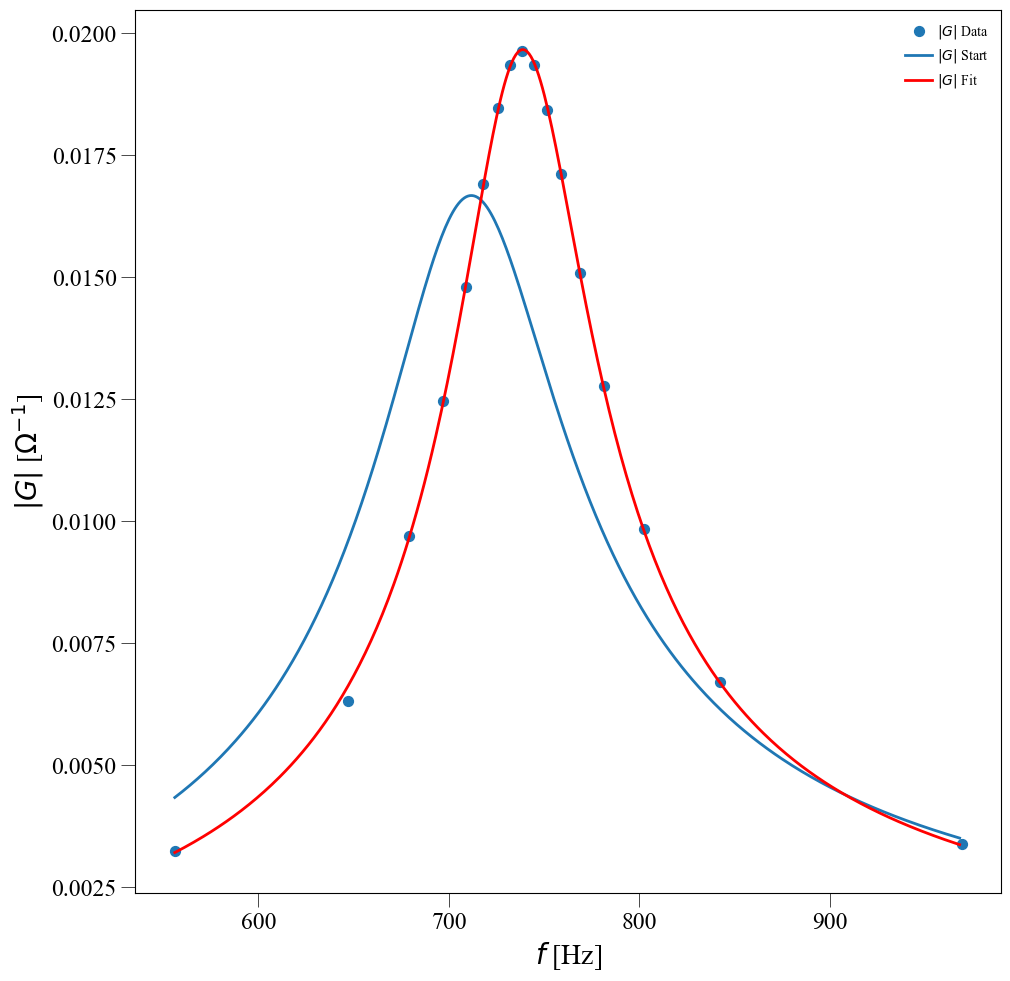
\includegraphics[scale=0.3]{G}
                \captionsetup{justification=centering, font=footnotesize}
                \captionof{figure}{Závislost amplitudy vodivosti $\vert G\vert$ na frekvenci $f$.}
                \label{fig:G}
                \raggedright
\end{minipage}
\newpage
\begin{minipage}[t]{0.5\textwidth} 
                \par \centering
                \vspace{10pt}
                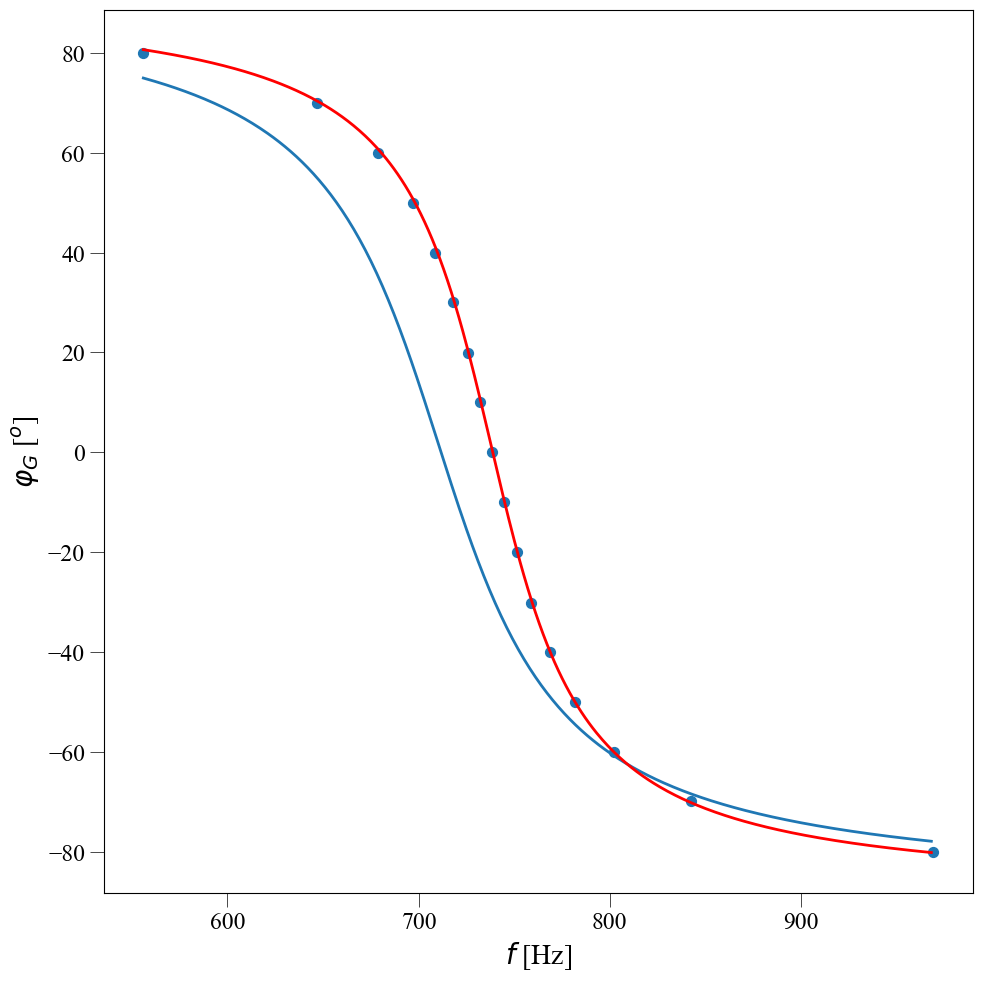
\includegraphics[scale=0.3]{phi_G}
                \captionsetup{justification=centering, font=footnotesize}
                \captionof{figure}{Závislost fáze amplitudy vodivosti $\varphi_G$ na frekvenci $f$.}
                \label{fig:phi_G}
                \vspace{10pt}
                \raggedright
                Data byla aproximována pomocí kódu $06RLCFitovaciPrikladPython3p8.zip$. Z aproximace byly získány následující hodnoty $R$ a $\omega_0$ a $\alpha$: 
                \begin{center}
                    $R$ = 50.9(4) [$\Omega$]
                    \vspace{5pt}
                    \par $\omega_0$ = 4642(1) [$\frac{rad}{s}$]
                    \vspace{5pt}
                    \par $\alpha$ = 221(1) [$s^{-1}$]
                \end{center}
                Proto podle vzorce (10) najdeme $L$ a podle vzorce (8) najdeme $C$:
                \begin{center}
                    $L$ = 115.3(6) [mH]
                    \vspace{5pt}
                    \par $C$ = 403(2)[nF]
                \end{center}
                Podle vzorce (9) nalezneme $F$:
                \begin{center}
                    $F$ = 8.67(4) [mH$^{-1}$]
                \end{center}
                Hodnota $f_0$ se získá ze vzorce (7): 
                \begin{center}
                    $f_0$ = 738.8(2) [Hz]
                \end{center}
                Hodnota Q se získá ze vzorce (11): 
                \begin{center}
                    $Q$ = 10.40(7)
                \end{center}
                Hodnota $R_{celk}$ pro $f_0$ se získá ze vzorce (13): 
                \begin{center}
                    $R_{celk}(f_0)$ = 50.83
                \end{center}
                Teoretické hodnoty $\omega_0$, $\alpha_0$, $F$, $f_0$ a $Q$ se rovnají:
                \begin{center}
                    $\omega_0$ = (4636 $\pm$ 30) [$\frac{rad}{s}$]
                    \vspace{5pt}
                    \par $\alpha$ = 223(2) [$s^{-1}$]
                    \vspace{5pt}
                    \par $F$ = 8.77(9) [mH$^{-1}$]
                    \vspace{5pt}
                    \par $f_0$ = 738(5) [Hz]
                    \vspace{5pt}
                    \par $Q$ = 10.4(3)
                    \vspace{5pt}
                \end{center}
\end{minipage}
\hspace{10pt}
\begin{minipage}[t]{0.5\textwidth} 
            \subsection{Přechodný jev RLC obvodu}
                Dále jsme použili zapojení obvodu na obrázku (\ref{fig:imp2}). 
                \par Měřili jsme podkritické, kritické a nadkritické tlumení. Příslušné použité odpory jsou následující: $R_{R,1}$ $R_{R,2}$ $R_{R,3}$.
                \par Pro podkritický tlumení byl získán následující graf závislosti napětí $U_2$ na době tlumení $t$: 
                \par \centering
                \vspace{10pt}
                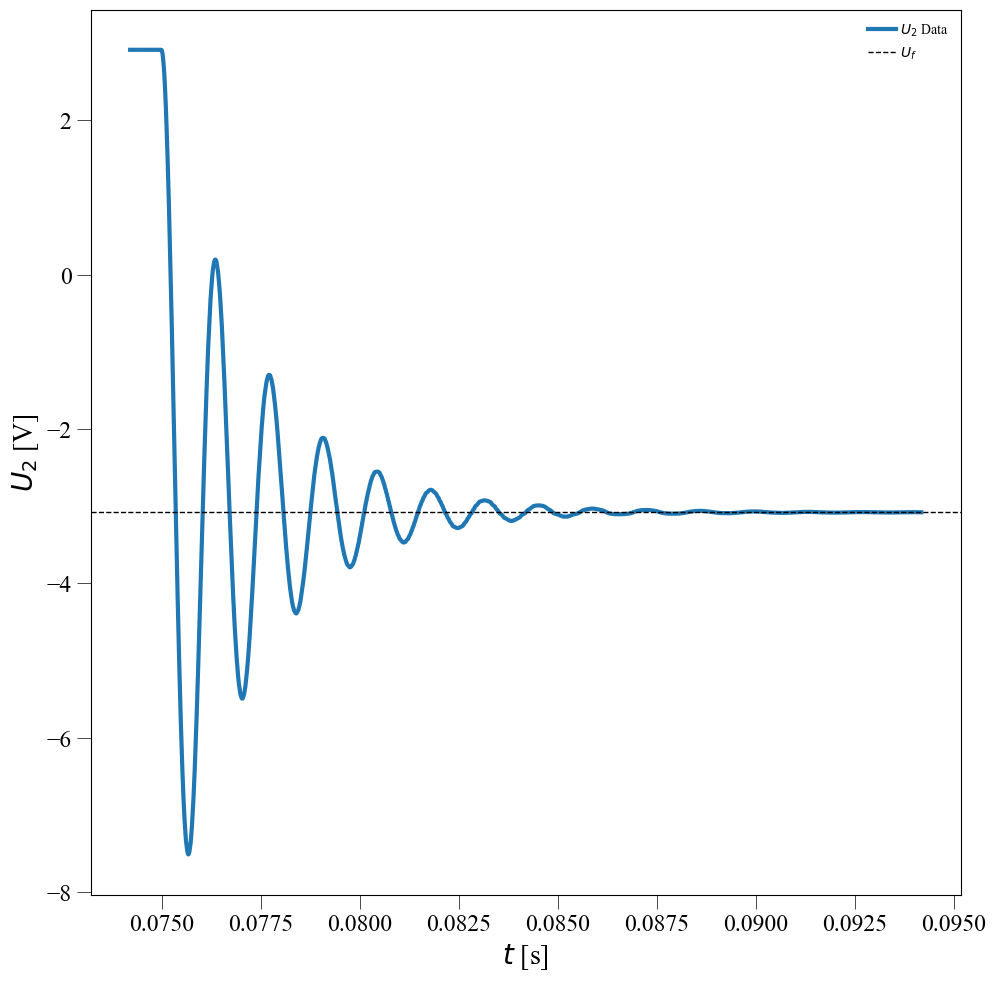
\includegraphics[scale=0.3]{pod_krit}
                \captionsetup{justification=centering, font=footnotesize}
                \captionof{figure}{Závislost napětí $U_2$ na době tlumení $t$ pro podkritický tlumení.}
                \label{fig:pod_krit}
                \raggedright
                \vspace{10pt}
                \par Z toho vyplývá, že konečné napětí $U_f$ je rovno: 
                \begin{center}
                    $U_f$ = -3.1 [V]
                \end{center}
                Dále vykreslíme závislost logaritmu rozdílu mezi maximy tlumení $ln(U_C-U_f)$ na době tlumení $t$ a lineárně ji aproximujeme: 
                \par \centering
                \vspace{10pt}
                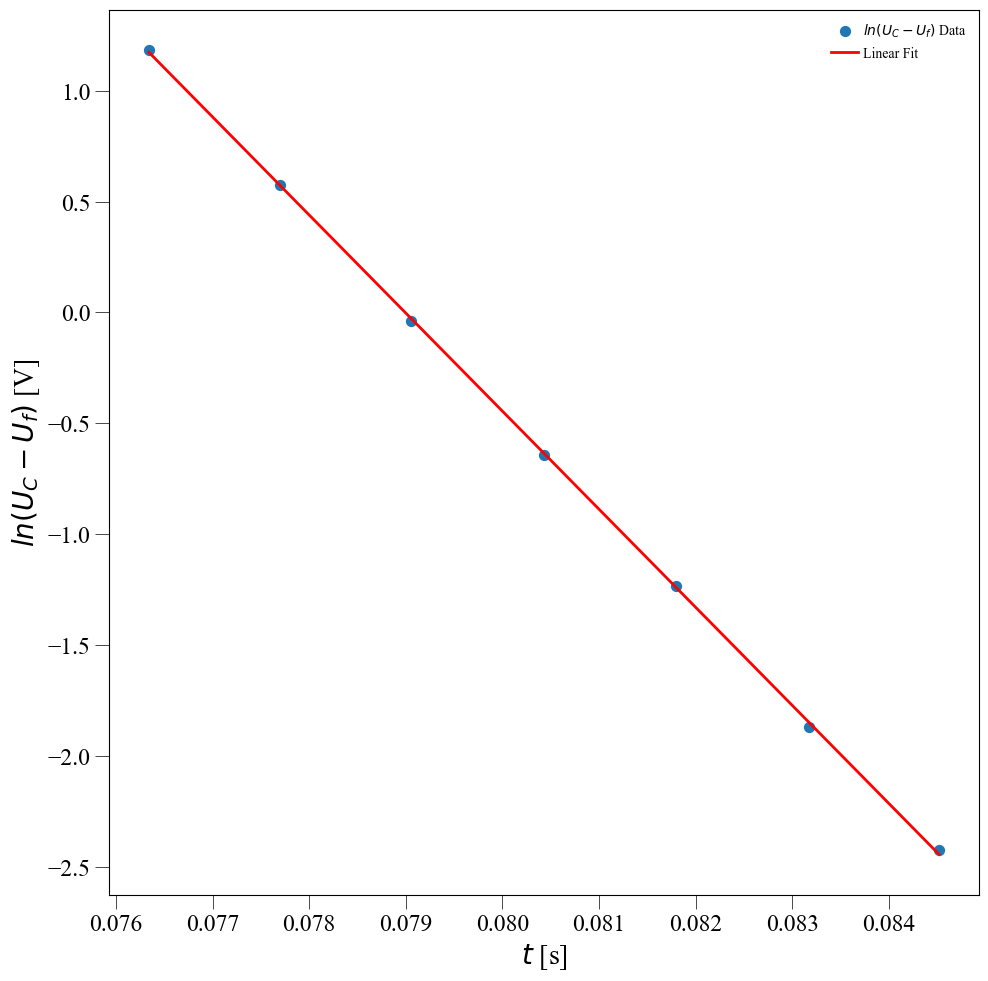
\includegraphics[scale=0.3]{pod_krit_fit}
                \captionsetup{justification=centering, font=footnotesize}
                \captionof{figure}{Závislost logaritmu rozdílu mezi maximy útlumu tlumení $ln(U_C-U_f)$ na době tlumení $t$ a jeho lineární aproximace.}
                \label{fig:pod_krit_fit}
                \raggedright
                \vspace{10pt}
\end{minipage}
\newpage
\begin{minipage}[t]{0.5\textwidth} 
                Z aproximace získáme hodnotu $\alpha$: 
                \begin{center}
                    $\alpha$ = 442(2) [$s^{-1}$]
                \end{center}
                Odpor obvodu $R$ se zjistí ze vzorce (10) pomocí známé hodnoty indukčnosti $L$:
                \begin{center}
                    $R_1$ = 101(1) [$\Omega$]
                \end{center}
                Proto podle vzorce (14) zjistíme tlumenou frekvenci oscilací $\omega_d$:
                \begin{center}
                    $\omega_d$ = 4621(1) [$\frac{rad}{s}$]
                \end{center}
                Najdeme teoretickou hodnotu rezonanční frekvence $f_0$ vydělením $\omega_0$ číslem $2 \pi$:
                \begin{center}
                    $f_0$ = 738.8(2) [Hz]
                \end{center}
                Známý použitý odpor $R_{R,1}$ = 29.12 [$\Omega$]. Známe také odpor $R_G$ = 50 [$\Omega$]. Odtud zjistíme $R_{celk, R1}$ a $R_{celk, R1} + R_G$ podle vzorce (13):
                \begin{center}
                    $R_{celk, R1}$ = 50 [$\Omega$]
                    \vspace{5pt}
                    \par $R_{celk, R1} + R_G$ = 100 [$\Omega$]
                \end{center}
                Pro kritický tlumení byl získán následující graf závislosti napětí $U_2$ na době tlumení $t$:
                \par \centering
                \vspace{10pt}
                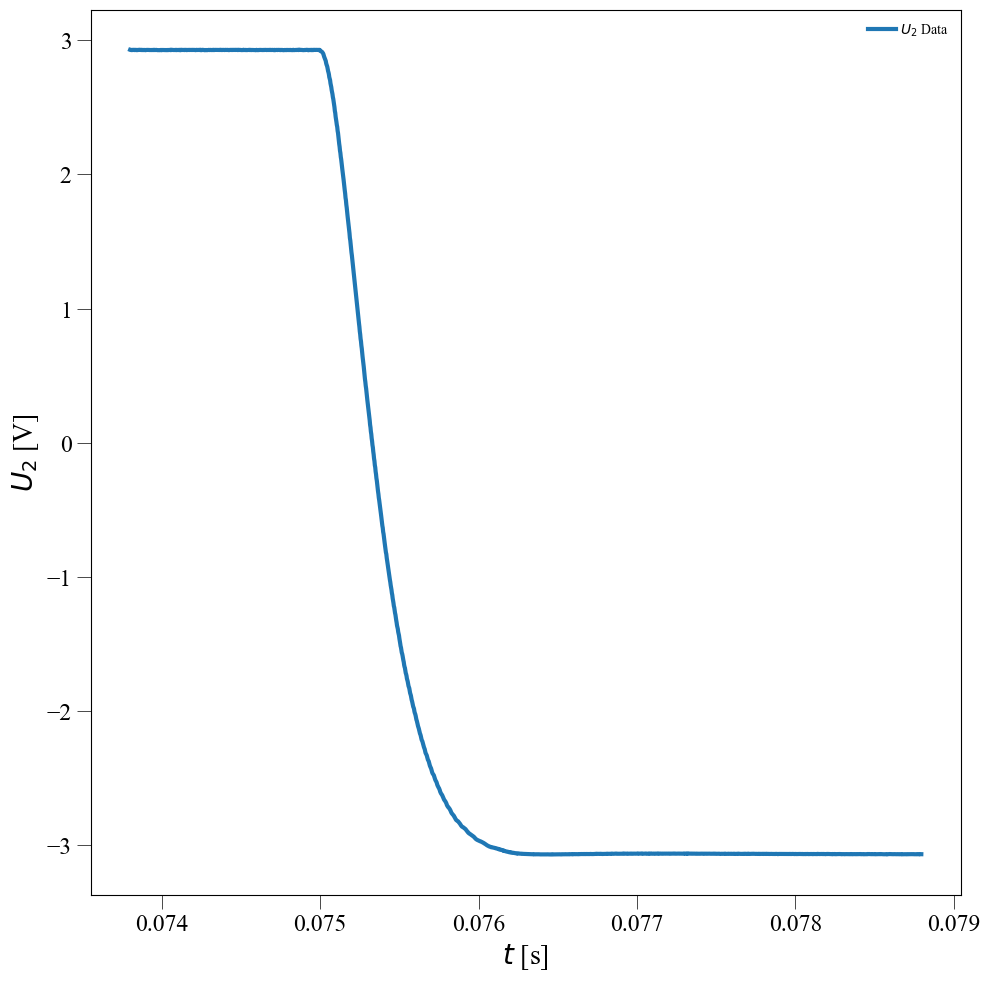
\includegraphics[scale=0.3]{krit}
                \captionsetup{justification=centering, font=footnotesize}
                \captionof{figure}{Závislost napětí $U_2$ na době tlumení $t$ pro kritický tlumení.}
                \label{fig:krit}
                \raggedright
                \vspace{10pt}
                Podle vzorce (16) zjistíme odpor obvodu $R_k$: 
                \begin{center}
                    $R_k$ = (1058 $\pm$ 10) [$\Omega$]
                \end{center}
\end{minipage}
\hspace{10pt}
\begin{minipage}[t]{0.5\textwidth} 
                Známý použitý odpor $R_{R,2}$ = 848.8 [$\Omega$]. Odtud zjistíme $R_{celk, R2}$ a $R_{celk, R2} + R_G$ podle vzorce (13):
                \begin{center}
                    $R_{celk, R2}$ = 870 [$\Omega$]
                    \vspace{5pt}
                    \par $R_{celk, R2} + R_G$ = 930 [$\Omega$]
                \end{center}
                Pro nadkritické tlumení byl získán následující graf závislosti napětí $U_2$ na době tlumení $t$: 
                \par \centering
                \vspace{10pt}
                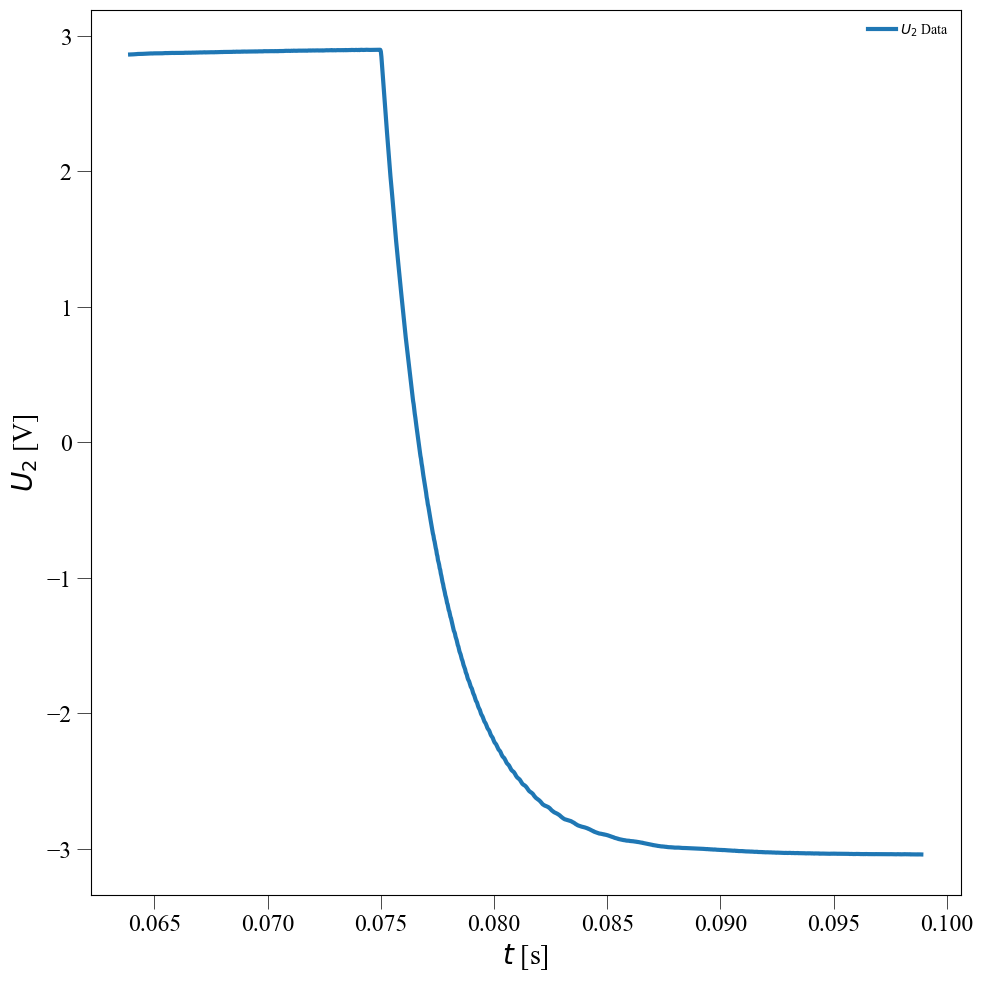
\includegraphics[scale=0.3]{nad_krit}
                \captionsetup{justification=centering, font=footnotesize}
                \captionof{figure}{Závislost napětí $U_2$ na době tlumení $t$ pro nadkritické tlumení.}
                \label{fig:nad_krit}
                \raggedright
                \vspace{10pt}
                Dále vykreslíme závislost logaritmu rozdílu mezi maximy nadkritického tlumení $ln(U_C-U_f)$ na době nadkritického $t$ a lineárně ji aproximujeme: 
                \par \centering
                \vspace{10pt}
                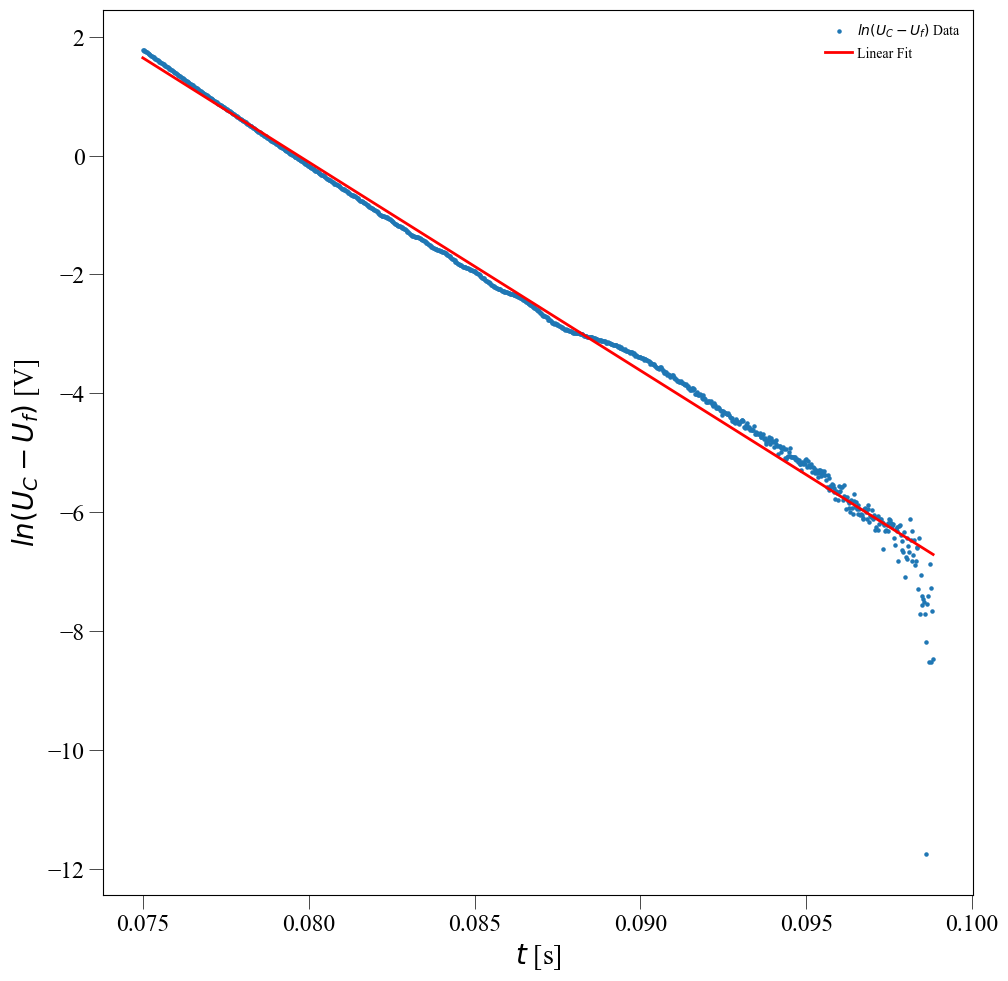
\includegraphics[scale=0.3]{nad_krit_fit}
                \captionsetup{justification=centering, font=footnotesize}
                \captionof{figure}{Závislost logaritmu rozdílu mezi maximy nadkritického tlumení $ln(U_C-U_f)$ na době nadkritického tlumení $t$ a jeho lineární aproximace.}
                \label{fig:nad_krit_fit}
                \raggedright
                \vspace{10pt}
\end{minipage}
\newpage
\begin{minipage}[t]{0.5\textwidth} 
                Získáme tedy hodnotu $\lambda_1$:
                \begin{center}
                    $\lambda_1$ = 351(1) [$s^{-1}$]
                \end{center}
                Pak odpor při nadkritickém tlumení $R_3$ zjistíme podle vzorce (18):
                \begin{center}
                    $R_3$ = (7050 $\pm$ 80) [$\Omega$]
                \end{center}
                Známý použitý odpor $R_{R,3}$ = 6002 [$\Omega$]. Odtud zjistíme $R_{celk, R3}$ a $R_{celk, R3} + R_G$ podle vzorce (13):
                \begin{center}
                    $R_{celk, R3}$ = 6023 [$\Omega$]
                    \vspace{5pt}
                    \par $R_{celk, R3} + R_G$ = 6073 [$\Omega$]
                \end{center}
                K výpočtu veličin a jejich nejistot byla použita knihovna Uncertinties pro Python: \href{pypi.org/project/uncertainties}. Kód je přiložen k protokolu. 
        \section{Závěr}  
            \subsection{Impedance}
                Hodnoty dekádového odporu naměřené multimetrem $R_R$ = 29.1 [$\Omega$] a osciloskopem $R_R$ = 29.72(2) [$\Omega$] se vzájemně shodují. Totéž lze říci o kapacitě kondenzátoru $C$ = 409.5 [nF] a $C$ = 408(4) [nF] a indukčnosti cívky $L$ = 113 [mF] a $L$ = 114(1) [mH].
            \subsection{Frekvenční charakteristika obvodu RLC}
                Hodnota odporu obvodu $R$ = 50.9(4) [$\Omega$] získaná měřením se téměř zcela shoduje s teoretickým výpočtem $R_{celk}(f_0)$ = 50.83. Hodnoty úhlové frekvence $\omega_0$ = 4642(1) [$\frac{rad}{s}$] se rovněž shodují s teoretickými hodnotami $\omega_0$ = (4636 $\pm$ 30) [$\frac{rad}{s}$]. Totéž lze říci o konstantě útlumu $\alpha$ = 221(1) [$s^{-1}$] a $\alpha$ = 223(2) [$s^{-1}$]. Kapacita kondenzátoru $C$ = 403(2)[nF] a indukčnost $L$ = 115.3(6) [mH] cívky rovněž dobře konvergují s dříve provedenými měřeními $C$ = 408(4) [nF] a $L$ = 114(1) [mH]. Naměřená hodnota oscilační síly $F$ = 8.67(4) [mH$^{-1}$] se rovněž shodují s teoretickými hodnotami $F$ = 8.77(9) [mH$^{-1}$]. Koeficient jakosti $Q$ = 10.40(7) se téměř rovná teoretickému $Q$ = 10.4(3). Naměřená frekvence $f_0$ = 738.8(2) [Hz] se prakticky neliší od původně stanovené $f_0$ = 738(5) [Hz].
\end{minipage}
\hspace{10pt}
\begin{minipage}[t]{0.5\textwidth} 
            \subsection{Přechodný jev RLC obvodu}
                Tlumicí konstanta pro podkritické tlumení z aproximace je $\alpha$ = 442(2) [$s^{-1}$]. Odpor obvodu $R_1$ = 101(1) [$\Omega$] konverguje k hodnotě $R_{celk, R1} + R_G$ = 100 [$\Omega$]. Tlumicí frekvence oscilací a úhlová frekvence oscilací jsou rovny $\omega_d$ = 4621(1) [$\frac{rad}{s}$], resp. $\omega_0$ = 4642(1) [$\frac{rad}{s}$]. Rezonanční frekvence je rovna $f_0$ = 738.8(2) [Hz].
                \par Při kritickém tlumení je odpor obvodu $R_k$ = (1058 $\pm$ 10) [$\Omega$], který se liší, ale je řádově stejný jako $R_{celk, R2} + R_G$ = 930 [$\Omega$].
                \par Pro nadkritický útlum je činitel poklesu z aproximace $\lambda_1$ = 351(1) [$s^{-1}$]. Odpor obvodu je $R_3$ = (7050 $\pm$ 80) [$\Omega$], který se výrazně liší, ale je ve stejném řádu velikosti jako $R_{celk, R3} + R_G$ = 6073 [$\Omega$]. Tento rozdíl může být způsoben nepřesností měření $\lambda_1$.
\end{minipage}
\newpage 
    \par K výpočtu chyb byl použit následující kód: 
    \begin{lstlisting}[language=Python, basicstyle=\tiny, breaklines=true]
        #Importing the libraries

        import matplotlib.pyplot as plt
        import numpy as np
        import pandas as pd
        from scipy import stats
        from scipy.optimize import curve_fit
        import uncertainties as u 
        from uncertainties import ufloat
        from uncertainties.umath import *
        from uncertainties import unumpy
        from lmfit import Minimizer, Parameters, fit_report

        # Constants and values

        R_I = 10.622 #Ohm

        #Reading data

        R_1 = pd.read_excel('R_1.xlsx')
        C_1 = pd.read_excel('C_1.xlsx')
        L_1 = pd.read_excel('L_1.xlsx')
        
        f_2 = pd.read_excel('f_2.xlsx')
        
        scope_0 = pd.read_csv('scope_0.csv')
        scope_1 = pd.read_csv('scope_1.csv')
        scope_2 = pd.read_csv('scope_2.csv')

        #Calculations

        R_1['U_20'] = R_1['U_20']*10**(-3)
        C_1['U_20'] = C_1['U_20']*10**(-3)
        L_1['U_20'] = L_1['U_20']*10**(-3)
        
        R_1['Z'] = R_I * R_1['U_M0']/R_1['U_20']
        C_1['Z'] = R_I * C_1['U_M0']/C_1['U_20']
        L_1['Z'] = R_I * L_1['U_M0']/L_1['U_20']
        
        C_1['C'] = -1/(2*np.pi*C_1['f']*C_1['Z']*np.sin(np.radians(C_1['phi'])))
        C_1['R'] = C_1['Z']*np.cos(np.radians(C_1['phi']))
        
        L_1['L'] = L_1['Z']*np.sin(np.radians(L_1['phi']))/(2*np.pi*L_1['f'])
        L_1['R'] = L_1['Z']*np.cos(np.radians(L_1['phi']))
        
        # print(R_1)
        # print(C_1)
        # print(L_1)
        
        R_1_mean = ufloat(R_1['Z'].mean(), np.std(np.array(R_1['Z'])))
        C_1_mean = ufloat(C_1['C'].mean(), np.std(np.array(C_1['C'])))
        L_1_mean = ufloat(L_1['L'].mean(), np.std(np.array(L_1['L'])))
        
        print('R_1=', R_1_mean)
        print('C_1=', C_1_mean)
        print('L_1=', L_1_mean)
        
        f_2['U_20'] = f_2['U_20']*10**(-3)
        
        f_2['Z'] = R_I * f_2['U_M0']/f_2['U_20']
        f_2['G'] = 1/f_2['Z']
        f_2['phi_G'] = -f_2['phi']
        
        # print(f_2)

        def G_teor(f_teor, R_teor, L_teor, C_teor):
            omega = 2*np.pi*f_teor
            return 1 / (np.sqrt(R_teor**2 + (omega*L_teor.nominal_value - 1/(omega*C_teor.nominal_value))**2))

        def phi_G_teor(f_teor, R_teor, L_teor, C_teor):
            omega = 2*np.pi*f_teor
            return np.degrees(np.arctan((1/(omega*C_teor.nominal_value)-(omega*L_teor.nominal_value))/R_teor))
        
        
        f_teor = np.linspace(556.100, 969.100, 1000)
        R_teor = R_1['Z'][2] + C_1['R'][2] + L_1['R'][2]
        L_teor = L_1_mean
        C_teor = C_1_mean
        
        alpha_teor = R_teor/(2*L_teor)
        omega_teor = 1/sqrt(L_teor*C_teor)
        F_teor = 1 / L_teor
        Q_teor = (L_teor*omega_teor)/R_teor
        f_0_teor = 1/(2*np.pi*sqrt(L_teor*C_teor))
        
        
        print('alpha_teor=', alpha_teor)
        print('omega_teor=', omega_teor)
        print('F_teor=', F_teor)
        print('Q_teor=', Q_teor)
        print('R_celk=', R_teor)
        print('f_0_teor=', f_0_teor)
        
        G_teor_values = G_teor(f_teor, R_teor, L_teor, C_teor)
        phi_G_teor_values = phi_G_teor(f_teor, R_teor, L_teor, C_teor)

        #RLC fit

        def Gabs(F,omega0,alpha,omega):
        	return omega*F/np.sqrt((omega0**2-omega**2)**2+(2*alpha*omega)**2)
        def Gphi(omega0,alpha,omega):  #faze ve stupnich
        	return np.arctan((omega0**2-omega**2)/(2*alpha*omega))/np.pi*180
        def residual(pars, omega, Gdata):
        	return Gabs(pars['F'],pars['omega0'],pars['alpha'],omega) - Gdata 
        
        fdata=f_2['f']
        odata=fdata*2*np.pi 
        Gdata=f_2['G']
        Phase=f_2['phi_G']
        
        R=60
        L=0.100
        C=500E-9
        
        ParsStart = Parameters()  
        ParsStart.add('F', value=1/L,vary=True)   
        ParsStart.add('omega0', value=1/np.sqrt(L*C),vary=True)  
        ParsStart.add('alpha', value=R/(2*L),vary=True)
        
        minner = Minimizer(residual, ParsStart, fcn_args=(odata,Gdata))
        results = minner.minimize() 
        ParsFit= results.params 
        
        print(fit_report(results))
        # FileStatistika= open('Statistika.dat', 'w+')
        # print(fit_report(results),file=FileStatistika)
        # FileStatistika.close()
        
        F=ufloat(ParsFit['F'], ParsFit['F'].stderr)  
        omega0=ufloat(ParsFit['omega0'], ParsFit['omega0'].stderr)
        alpha=ufloat(ParsFit['alpha'], ParsFit['alpha'].stderr)
        
        L=1/F
        R=2*L*alpha
        C=1/(L*omega0**2)
        Q=omega0/(2*alpha)
        f0=omega0/(2*np.pi)
        print("R=", R,"Ohm, L=", L*1000,"mH, C=", C*1E9,"nF,  Q=",Q, "f0=", f0, "Hz")
        
        ftheor = np.arange(np.amin(fdata), np.amax(fdata), 1)
        otheor=ftheor*2*np.pi
        
        GabsStart = Gabs(ParsStart["F"],ParsStart["omega0"],ParsStart["alpha"],otheor)  
        GphiStart = Gphi(ParsStart["omega0"],ParsStart["alpha"],otheor) 
        GabsFit = Gabs(ParsFit["F"],ParsFit["omega0"],ParsFit["alpha"],otheor)  
        GphiFit = Gphi(ParsFit["omega0"],ParsFit["alpha"],otheor) 
        
        # FileFitSpekta= open('FitSpekta.dat', 'w+')
        # print ("f[Hz]", "\t", "GabsStart",  "\t", "GphiStart", "\t", "GabsFit",  "\t", "GphiFit", file=FileFitSpekta)
        # for i in range(len(ftheor)):
        #     print (ftheor[i],"\t",GabsStart[i],  "\t",GphiStart[i], "\t", GabsFit[i],  "\t",GphiFit[i], file=FileFitSpekta)
        # FileFitSpekta.close()


        R_measur = R
        omega_measur = omega0
        alpha = alpha
        L_measur = L*1000
        C_measur = C*1E9
        F_measur = F
        f_0_measur = f0
        Q_measur = Q

        # #Linear fitting

        u_c_list = [0.18965242, -1.29941085, -2.11729032, -2.5510466, -2.78644109, -2.92356013, -2.98914254]
        ln_u_list = np.log(u_c_list-u_f)
        t_c_list = [0.07634, 0.0777, 0.07905, 0.08043, 0.0818, 0.08317, 0.08452]
        
        # Calculate linear regression parameters
        slope, intercept, r_value, p_value, std_err = stats.linregress(t_c_list, ln_u_list)
        alpha_d = ufloat(np.abs(slope), np.abs(std_err))
        print('alpha_d =', alpha_d)
        
        # Create the best-fit line
        best_fit_line = slope * np.array(t_c_list) + intercept

        R_G = 50
        R_R_1 = 29.12
        R_R_2 = 848.8
        R_R_3 = 6002
        
        R_1_3 = alpha_d*2*L_1_mean
        
        omega_d = sqrt(omega_measur**2 - alpha_d**2)
        
        f_0_3 = omega_measur / (2 * np.pi)
        
        R_celk_1 = R_R_1 + C_1['R'][2] + L_1['R'][2]
        R_celk_2 = R_R_2 + C_1['R'][2] + L_1['R'][2]
        R_celk_3 = R_R_3 + C_1['R'][2] + L_1['R'][2]
        
        R_2_3 = 2 * omega_measur * L_1_mean
        
        print('R_celk_1 =', R_celk_1)
        print('R_celk_2 =', R_celk_2)
        print('R_celk_3 =', R_celk_3)
        
        print('f_0_3 =', f_0_3)
        print('R_1_3 =', R_1_3)
        print('R_2_3 =', R_2_3)
        print('omega_d =', omega_d)

        #Linear fitting
        u_c_list_2 = scope_2['u_2'][443:1397]
        u_f_2 = -3.04138675
        
        ln_u_list_2 = np.log(u_c_list_2 - u_f_2)
        
        # Calculate linear regression parameters
        slope, intercept, r_value, p_value, std_err = stats.linregress(scope_2['t'][443:1397], ln_u_list_2)
        lambda_1 = ufloat(np.abs(slope), np.abs(std_err))
        print('lambda_1 =', lambda_1)
        
        # Create the best-fit line
        best_fit_line = slope * np.array(scope_2['t'][443:1397]) + intercept

        R_3_3 = -L_1_mean * ((omega_measur**2 + lambda_1**2) / lambda_1) 
        print('R_3_3 =', R_3_3)
    \end{lstlisting} 
\end{document}